% !TEX root = ../my-thesis.tex
%
\chapter{State of the Art}
\label{sec:sota_2}

\cleanchapterquote{Qual è 'l geometra che tutto s'affige; per misurar lo cerchio, e non ritrova; pensando, quel principio ond'elli indige. Tal era io a quella vista nova: 
veder voleva come si convenne; l'imago al cerchio e come vi s'indova. }{Dante Alighieri}{(Italian poet, 1265-1321)}

In this section we delve deeper into the theory of emulators, and discuss the state of the art in the field. In this manuscript, we have first encountered the use of emulators in the context of \gls{gpr} in \S\ref{sec:ntools:gpr}, when building a surrogate model for the \gls{cmp} hyperparameters in \S\ref{sec:surr} and when building a surrogate model for the \gls{cfd} codes in \S\ref{sec:cfd}.
\blue{In this chapter, we will focus on the problem of building surrogate models for discontinuous functions, which is a well-known challenge in the field of surrogate modeling. We will discuss existing approaches for surrogating discontinuous functions and present a novel data-driven approach that is able to build a piecewise representation of the function.}

\section{Emulation of Computer Codes}

The field of computer emulation, often referred to as surrogate modeling, emerged from the need to analyze highly complex, computationally expensive computer simulations. In particular, the field of \gls{uq} relies heavily on emulators since computations often require many model evaluations, which can be prohibitively expensive when using the original computer code. By building simple, cheap-to-evaluate probability models (emulators), practitioners were finally able to thoroughly explore vast parameter spaces that were previously inaccessible~\cite{santner2003}. The field has since evolved into a rich and diverse area of research, encompassing a wide range of techniques and applications, from engineering design optimization to climate modeling and beyond.

\smallskip
The foundations of this methodology were heavily inspired by traditional regression techniques, which historically relied on experimental data to model the behavior of real-world systems. Just as traditional scientists needed a systematic way to gather data, a practice pioneered as the \gls{doe}~\cite{fisher1925}, computational scientists required their own sampling strategies, leading to the birth of \textit{computer experiments} and \gls{ndoe}~\cite{mckay1979}. In \S\ref{sec:sota_1}, we have already hinted at this similarity when discussing the art of calibration. In particular, we said that calibration can be used to estimate plausible values of physical parameters using real-world data, or to build emulators using computer-generated data. In this regard, let us reference the calibration equation for an emulator, which is just a restatement of Eq.~\eqref{eq:sota_1:caleq}:

\begin{equation}
\label{eq:sota_2:caleq}
f_i = \tilde{f}(\mathbf{x}_i; \boldsymbol{\beta}) + \eta_i \;.
\end{equation}

In Eq.~\eqref{eq:sota_2:caleq}, the set $\data = \{(\bx_i, f_i)\}_{i=1}^{\nobs}$ represents the \gls{ndoe}, \blue{with $\bx_i$ the input and $f_i$ the output}, and $\tilde{f}(\cdot) : \mathbb{R}^d \to \mathbb{R}$ is the emulator, whose response function is parameterized by some hyperparameters $\boldsymbol{\beta}$. The fundamental difference between the two calibration problems is that in the case of computer emulation, the data $\data$ is generated by running the computer code at different input settings $\bx_i$, while in the case of physical calibration, the data is obtained from real-world experiments. This distinction has profound implications for how we model and analyze the data, as well as for the types of uncertainties we need to consider. Traditional statistical methods, such as response surface methodology~\cite{box1951}, were designed to account for random measurement errors inherent in physical experiments. In contrast, computer experiments are typically deterministic; running the exact same code with the same inputs yields the exact same output. This lack of random error required a paradigm shift in statistical modeling, moving away from traditional regression toward spatial modeling techniques, like \gls{gpr}, specifically tailored for computer codes~\cite{sacks1989}. The term $\eta_i$ in Eq.~\eqref{eq:sota_2:caleq} is often referred to as the \textit{nugget} term, and it is used to account for numerical noise or other sources of variability that may arise in computer simulations, such as convergence issues or stochastic elements within the code. This nugget term is modeled as a Gaussian random variable $\eta_i \sim \mathcal{N}(0, \sigma_n^2)$; however, in many cases, especially when dealing with deterministic computer codes, this term is set to zero, reflecting the fact that there is no inherent randomness in the outputs. 

\smallskip
In the previous chapters, we have already touched upon some of the most interesting research questions in the field of computer emulation, such as how to find the value of the hyperparameters $\boldsymbol{\beta}$, and how to design the \gls{ndoe} $\data$. In this chapter, we shall focus on the question of choosing the right model for the emulator $\tilde{f}(\cdot)$. 

\smallskip
To lay the groundwork for this discussion, let us formally recall how a parametrized computer model is typically structured via the following abstract system of equations:

\begin{equation}
\label{eq:sota_2:compmod}
\left\{ 
\begin{aligned}
&\mathcal{M}(\mathbf{u}; \mathbf{x}) = 0 \\
&f(\mathbf{x}) = \mathcal{O}(\mathbf{u}; \mathbf{x}) \;.
\end{aligned}
\right.
\end{equation}

In Eq.~\eqref{eq:sota_2:compmod}, the vector $\mathbf{x} \in \Omega \subset \mathbb{R}^{d_x}$ represents the input parameter space, while the operator $\mathcal{M}(\cdot)$ represents the underlying mathematical model, which is frequently expressed as a highly non-linear system of \glspl{pde}~\cite{quarteroni1994numerical}. The solution to this mathematical model, $\mathbf{u}(\mathbf{x})$, lives in a Hilbert space $H$, and $\mathcal{O}: H \times \Omega \rightarrow \mathbb{R}$ is an observation operator that extracts a specific \gls{qoi}, denoted as $f(\mathbf{x})$, from the system state $\mathbf{u}$~\cite{quarteroni1994numerical}. In the realm of machine learning and computational methods, two main schools of thought have emerged to build fast emulators for these expensive computer codes.

\smallskip
\subsection{Reduced Order Models}
On the one hand, intrusive methods, such as projection-based \glspl{rom}, build a reduced-order version of the physical operator $\mathcal{M}$, here called $\mathcal{M}_{\mathrm{ROM}}$, by assuming that the solution manifold can be accurately embedded within a low-dimensional linear subspace $H_{\mathrm{ROM}} \subset H$~\cite{rom_1}. The full-order equations are mapped onto this subspace using mathematically rigorous projections, such as orthogonal and oblique projections~\cite{Fick2017, FarhatOblique}. The solution to the simplified problem, here termed $\mathbf{u}_{\mathrm{ROM}}$, is then passed through the observation operator $\mathcal{O}$ to obtain an approximation of $f$. In the field of \gls{cfd}, \glspl{rom} are a well-established tool for building fast surrogates of complex fluid flows, and have been successfully applied to a wide range of problems, from aerodynamic design optimization to real-time control of turbulent flows~\cite{Ruan2026, Frahat2008, Fick2018, Manzoni2012, Chen2017}. Practitioners highly praise the physical rigor of this approach and that one can freely change the observation operator $\mathcal{O}$ without re-computing the reduced order basis spanning~$H_{\mathrm{ROM}}$. Indeed, the bulk of the computational cost is generally associated with the inversion of $\model(\mathbf{u}; \mathbf{x}) = 0$, while the evaluation of $\mathcal{O}$ is typically negligible. Using a \gls{rom}, one can therefore obtain a fast surrogate for the full state $\mathbf{u}$, which can be used to compute any \gls{qoi} of interest.

\smallskip
\subsection{Black-box Emulators}
The main disadvantage of intrusive approaches is that they require direct manipulation of the governing equations $\model$~\cite{Padula2024}, which can be a significant barrier to entry for practitioners, as it often requires a deep understanding of the underlying physics and numerical methods, as well as access to and modifications of the source code of the full-order solver. 

\smallskip
A fundamentally different approach is therefore taken by non-intrusive, data-driven methods, which aim at \blue{approximating} the mapping from $\mathbf{x}$ to $f=f(\mathbf{x})$ directly, treating $\mathcal{M}$ entirely as a black box and data-generating process. Modeling the mapping from some inputs $\mathbf{x}$ to some observable $f$ using simple functions is a well-known problem in the field of regression. Although it is not easy to pinpoint the exact origin of this field (it mostly depends on what we can actually consider a surrogate model), we would like to mention the work of Lord Kelvin in the late 19th century, who used simple harmonic functions to model and predict the tidal patterns in the ocean~\cite{Tides}. Back then the tidal governing equations were fully known~\cite{pekeris1969}, but solving them was impossible. Restricting the definition of a surrogate model to the modern definition of computer emulation, the field of surrogate modeling can be traced back to the seminal work of Sacks et al.~\cite{sacks1989design}, who introduced the use of \gls{gpr} as a surrogate model for computer codes. Since then, the field has evolved rapidly, and a wide range of surrogate modeling techniques have been developed, including \gls{pce}~\cite{xiu2002wiener,Sudret2008}, \glspl{svm}~\cite{clarke2005analysis}, and \glspl{nn}~\cite{ghaboussi1991knowledge, Cuomo2022}, among many others.

\smallskip
Out of all these techniques, \gls{gpr} and \gls{pce} are the most widely used in the field of \gls{uq}, and are often considered the workhorses of surrogate modeling. They are very popular because they are well suited for \gls{uq} tasks, as they provide a probabilistic framework for modeling the uncertainty in the predictions, and they are relatively easy to train and interpret. Both \gls{gpr} and \gls{pce} can be expressed as a linear combination of $M$ basis functions, i.e., they can be written in the form:

\begin{equation}
    \tilde{f}(\mathbf{x}; \boldsymbol{\beta}) = \sum_{i=1}^{M} a_i(\boldsymbol{\beta}) \phi_i(\mathbf{x}; \boldsymbol{\beta}) \;,
    \label{eq:sota_2:lincomb}
\end{equation}

where $\{\phi_i\}_{i=1}^{M}$ are the basis functions, and $a_i$ are the coefficients of the expansion. Notice that the expansion is parameterized by some hyperparameters $\boldsymbol{\beta}$. Estimating these hyperparameters using some training data $\data$ is the main task of surrogate modeling, and is often referred to as \textit{model selection}~\cite{uq_theory}.

\smallskip
Although sharing some interesting similarities, \gls{pce} and \gls{gpr} are fundamentally different objects. In \gls{pce}, the basis functions $\{\phi_i\}$ are typically fixed and chosen to be orthogonal polynomials with respect to some measure on $\Omega$, and training corresponds to estimating the coefficients $a_i$ using some numerical quadrature or regression technique~\cite{Sudret2008}. This is particularly useful when one is interested in modeling random variables and their statistical moments, as the orthogonality property of the basis functions allows for the direct analytical computation of these quantities from the surrogate model~\cite{Sudret2008, Xiu2002}. 

\smallskip
In \gls{gpr}, the basis functions are not fixed, but are parameterized by the hyperparameters $\boldsymbol{\beta}$ of the covariance function. Conversely, the coefficients, once the hyperparameters are fixed, are not free parameters but are determined by the \gls{gp} equations; see our discussion in \S\ref{sec:ntools:gpr}. Training corresponds to estimating the hyperparameters $\boldsymbol{\beta}$ from the training data. \gls{gp} models are particularly useful when one is interested in modeling the uncertainty in the predictions, as they provide a natural way to quantify the uncertainty in the predictions through the posterior distribution over functions~\cite{uq_theory}.

\smallskip
Despite these profound differences, from the practitioner's point of view, training \glspl{gp} and \glspl{pce} involves maximizing a score function $S(\boldsymbol{\beta}, \data)$, which is a function of the hyperparameters $\boldsymbol{\beta}$. This score function is usually the log-marginal likelihood in the case of \gls{gpr}, Eq.~\eqref{eq:score_gp}, and the negative regularized \gls{mse} in the case of \gls{pce}, Eq.~\eqref{eq:score_pce}.

\begin{subequations}
\label{eq:sota_2:score_functions}
\begin{align}
    S_\mathrm{GP}(\boldsymbol{\beta}, \data) &= \log \mathrm{p}(\data \mid \boldsymbol{\beta}) \label{eq:score_gp} \\
    S_\mathrm{PCE}(\boldsymbol{\beta}, \data) &= -\frac{1}{2} \sum_{i=1}^{\nobs} \left( y_i - \boldsymbol{\phi}(\bx_i)^{\top} \boldsymbol{\beta} \right)^2 - R(\boldsymbol{\beta}) \label{eq:score_pce}
\end{align}
\end{subequations}

In Eq.~\eqref{eq:score_gp}, $\mathrm{p}(\data \mid \boldsymbol{\beta})$ is the marginal likelihood of the data given the hyperparameters $\boldsymbol{\beta}$, see \S\ref{sec:ntools:gpr} for more details, while $R(\boldsymbol{\beta})$ in Eq.~\eqref{eq:score_pce} is a regularization term that is often added to the \gls{pce} score function to prevent overfitting and $\boldsymbol{\phi}(\bx_i)$ is the vector of basis functions evaluated at $\bx_i$. Notice that the score functions in Eq.~\eqref{eq:sota_2:score_functions} are a function of the hyperparameters $\boldsymbol{\beta}$, and training corresponds to finding the value of $\boldsymbol{\beta}$ that maximizes this score function.

\smallskip
Specific optimization algorithms for maximizing the score functions in Eq.~\eqref{eq:sota_2:score_functions} have been developed for both classes of models, and are widely available in many software packages. These algorithms often come with automatic gradient computation, which can significantly speed up the optimization process, especially when dealing with high-dimensional hyperparameter spaces. 

\smallskip
\subsection{Hybrid Approaches}

A recent trend in the field of surrogate modeling is the development of hybrid approaches that combine the strengths of both intrusive and non-intrusive methods. These methods aim at learning a map $\mathcal{G}: X \rightarrow H$ between the input space $X$ and the solution space $H$, such that $\mathcal{M}(\mathcal{G}(\mathbf{x}); \mathbf{x}) \approx 0$. In this way, one can leverage the availability of the solution of the full-order model $\mathcal{G}(\bx) \approx \mathbf{u}$ with the flexibility of non-intrusive methods. A first approach in this direction is the use of so-called \textit{non-intrusive} \glspl{rom}, which are built by first generating a set of snapshots of the full-order solution $\mathbf{u}(\bx)$ at different input settings $\bx_i$, and then using these snapshots to build a reduced-order basis $H_{\mathrm{ROM}}$~\cite{rom_1}. Once the reduced-order basis is built, one can use non-intrusive methods, such as \gls{gpr}, to learn the mapping from $\bx$ to the coefficients of the reduced-order basis, and then use these coefficients to reconstruct the full-order solution $\mathbf{u}(\bx)$; see~\cite{hybrid_rom} for a very recent application of this approach.

\smallskip
Similarly, \textit{Operator Learning} techniques rely on deep learning to approximate the fundamental mapping $\mathcal{G}: X \rightarrow H$~\cite{Kovachki2023}. Rather than predicting a finite-dimensional \gls{qoi}, neural operators learn to map inputs $\bx$ directly to states $\mathbf{u}$~\cite{Kovachki2023, Lu2021}. Some works in this space, such as the Deep Operator Network~\cite{Lu2021, Goswami2022} and the Fourier Neural Operator (FNO)~\cite{Kovachki2023, Kovachki2021}, have demonstrated remarkable success in learning complex mappings for high-dimensional \glspl{pde}. A nice property of these methods is their discretization-invariance: because the operator is parameterized in continuous space, it enables \textit{zero-shot} super-resolution, allowing models trained on coarse grids to be instantly evaluated on highly refined meshes without retraining~\cite{Kovachki2023}.

\subsection{Scope of the Chapter}

\bigskip
In this chapter, we will focus only on non-intrusive, data-driven methods, leaving possible extensions to intrusive \glspl{rom} and neural operators for future work. An interesting question that arises in the context of non-intrusive surrogates is how to represent discontinuous functions, which are common in many physical systems, such as those involving shocks or phase transitions. Both \gls{pce} and \gls{gpr} struggle to capture discontinuities, as they are inherently designed to model smooth functions~\cite{uq_theory, Sudret2023, Palar2024}. \red{In the case of \gls{pce}, the struggle arises from the global and smooth nature of the basis functions. The presence of a discontinuity introduces a sharp trade-off: it either induces significant global errors if the dimensionality of the polynomial bases is insufficient, or triggers spurious oscillations near the discontinuity when high-degree polynomial bases are used. This phenomenon is known as \textit{Gibbs Oscillations}~\cite{uq_theory}. Similarly, \gls{gpr} struggles to emulate discontinuous functions because standard covariance functions are typically smooth and stationary. This formulation inherently assumes that the underlying function exhibits uniform, smooth behavior across the entire input space, an assumption that is violated by the presence of discontinuities, consequently leading to localized oscillations and suboptimal hyperparameter optimization.}

\blue{In the next sections, we will discuss a few approaches that have been proposed in the literature to address this challenge, and we will introduce a novel approach that combines clustering, classification and regression to build a piecewise surrogate model that can effectively capture discontinuities in the function $f$.}

\section{Representing Discontinuous Functions Using Piecewise Surrogate Models}
\label{sec:discontinuous_functions}

Dealing with discontinuous functions is a well-known challenge in the field of surrogate modeling. When the function $f$ exhibits discontinuities, two main problems arise: (i) Training the surrogate model becomes more difficult, and learned hyperparameters can be biased; (ii) The \gls{mse} of the surrogate model can be significantly higher even far from the discontinuity. Surely, complex surrogate models, such as neural networks~\cite{ziatdinov2024activelearningfullybayesian}, can be used to capture discontinuities but often require a large amount of training data and are less interpretable than simpler surrogate models, such as \gls{pce} and \gls{gpr}~\cite{Palar2024}.

\smallskip
In some cases, it is possible to use expert domain knowledge to identify the location of the discontinuity prior to building the surrogate model. For example, in~\cite{GoriGallia2024}, the authors propose a binary split of the training data according to a known regime indicator and then fit a local \gls{pce} regressor in the subdomain of interest. There are cases in which the discontinuity is not known a priori, but one can still rely on properties of the functions. In~\cite{Gori2022}, the authors propose to use a threshold approach to develop a non-linear \gls{pce} expansion for handling a regime change in the model response. As far as \glspl{gp} are concerned, the first approach to satisfy the need for more complex data representations was the introduction of non-stationary covariance functions, such as the Gibbs kernel~\cite{gibbs1997}, which allows for different length scales in different regions of the input space. By lowering the correlation length near a discontinuity, the model can also capture the behavior of the function in those regions. Since the extension of this work to multiple dimensions by~\cite{Paciorek2004}, the standard approach is to introduce a second \gls{gp} to model the length scale of the first \gls{gp}~\cite{Hinonen2016}, as done, for example, in~\cite{Chen2023}. A different approach to building more complex covariance functions for \gls{gpr} is proposed in~\cite{Sudret2023, palmatti2020}, in which the authors introduce a categorical variable in the \gls{gp} covariance function to indicate that a point belongs to a different dataset, thus allowing the model to capture discontinuities between the two datasets.

\smallskip
While these approaches have proved to be effective in some cases, they are often problem-specific, may require prior knowledge of the location of the discontinuity and can be computationally expensive to train, especially when dealing with high-dimensional input spaces or large datasets. 

\smallskip
It is therefore desirable to have a more general and \blue{automatic} approach that can handle discontinuities without requiring problem-specific knowledge or modifications to the structure of the surrogate model. A promising approach to achieve this is to consider a piecewise surrogate model, in which the input space $\Omega$ is partitioned into a disjoint union of subdomains $\Omega = \cup_{l=1}^L \Omega_l \text{ with } \Omega_l \cap \Omega_k = \emptyset \;\forall\; l \neq k$, and a local surrogate model $\tilde{f}_l$ is trained on each subdomain $\Omega_l$. The global surrogate model can then be defined as a piecewise function that combines the local surrogate models, i.e.,

\begin{equation}
    \tilde{f}(\mathbf{x}; \boldsymbol{\beta}, \mathcal{P}) = \sum_{l=1}^{L} \mathbb{I}_{\Omega_l}(\mathbf{x}) \tilde{f}(\bx; \boldsymbol{\beta}_l) \;.
    \label{eq:sota_2:f_piece_surr}
\end{equation}

Eq.~\eqref{eq:sota_2:f_piece_surr} introduces a new degree of freedom into the problem, which is the partition $\mathcal{P} = \{\Omega_l\}_{l=1}^L$ of the input space $\Omega$. \blue{Notice that the partition $\mathcal{P}$ is generally not known a priori, and must be learned from the training data $\data$.} 

The main advantage of \blue{a piecewise} approach is that it allows us to capture discontinuities in the function $f$ by training specialized local surrogate models $\tilde{f}(\cdot; \boldsymbol{\beta}_l)$ that are tailored to the local behavior of $f$ in each subdomain $\Omega_l$. This can significantly reduce the error of the surrogate model, as, thanks to the properties (additive and disjoint) of the partition $\mathcal{P}$, the error of the piecewise surrogate model can be decomposed as follows:

\begin{equation}
    \| f - \tilde{f} \|^2 = \sum_{l=1}^L \int_{\Omega_l} (f(\mathbf{x}) - \tilde{f}(\mathbf{x}; \boldsymbol{\beta}_l))^2 \mathbb{P}(\dd \mathbf{x})\;.
    \label{eq:sota_2:error_decomposition}
\end{equation}

Eq.~\eqref{eq:sota_2:error_decomposition} hints that if the partition $\mathcal{P}$ is chosen in such a way that the function $f$ is smooth within each subdomain $\Omega_l$, then the local surrogate models $\tilde{f}(\cdot; \boldsymbol{\beta}_l)$ can be trained to achieve a low error, thus leading to a low overall error for the piecewise surrogate model.

\smallskip
As a final remark, partitioning the input space $\Omega$, and eventually the training data $\data$, reduces the training cost of the surrogate model~\cite{konomi2019}, which can be a significant advantage when dealing with large datasets or high-dimensional input spaces. Indeed, training a global surrogate model has a cost that generally scales with the cube of the training set size $n$, while training $L$ local surrogate models has a cost that scales with the cube of the average training set size $n/L$, leading to a significant reduction in training time when $n$ is large.

\smallskip
The main challenge of this approach is jointly identifying a good partition $\mathcal{P}$ of the input space $\Omega$ and the hyperparameters $\boldsymbol{\beta}_l$ of the local surrogate models. In particular, one should first ask how to parameterize the huge space of all possible partitions of $\Omega$, and then how to actually explore it using only the training data $\data$. 

\smallskip
\blue{In a purely data-driven approach, one needs to identify the partition $\mathcal{P}$ and the hyperparameters $\boldsymbol{\beta}_l$ of the local surrogate models from the training data $\data$ alone. This is a complex problem that can be attacked by breaking it down by cleverly combining three common Machine Learning tasks: (i) Clustering, (ii) Classification and (iii) Regression. The remainder of this section is dedicated to a brief discussion of these techniques and an introduction to the notation adopted in the rest of the chapter.}

\smallskip
\blue{First, clustering is the task of partitioning the training data $\data$ into subsets, in a meaningful way~\cite{stats_pr}. In practice, it corresponds to assigning a latent variable $z_i \in \{1, \ldots, L\}$ to each training point $\mathbf{d}_i = (\bx_i, f_i) \in \data$. We call $\mathbf{z} = \{z_i\}_{i=1}^{\nobs}$ the vector of cluster labels. A cluster $\data_l$ is then defined as the set of training points that share the same cluster label $l$, i.e., $\data_l = \{\mathbf{d}_i \in \data : z_i = l\}$. Clustering is very useful to identify the partition $\mathcal{P}$ of the input space $\Omega$, as it allows us to group together training points that should belong to the same subdomain $\Omega_l$.}

\smallskip
\blue{Classification is the task of learning a map from the input space $\Omega$ to the cluster labels $\{1, \ldots, L\}$. In other words, classification is the task of training a classifier $c(\cdot, \boldsymbol{\gamma}): \Omega \to \{1, \ldots, L\}$ that can predict the cluster label $z$ for any input $\bx$ ($L$ is the number of clusters). The classifier is parameterized by some hyperparameters $\boldsymbol{\gamma}$, which can be trained using the available cluster labels $\mathbf{z}$ as training data. Once the classifier is trained, we can use it to define the partition $\mathcal{P}$ of the input space $\Omega$, by defining $\Omega_l = \{\bx \in \Omega : c(\bx; \boldsymbol{\gamma}) = l\}$.}

\smallskip
\blue{Finally, regression is the task of training a local surrogate model $\tilde{f}(\cdot; \boldsymbol{\beta}_l)$ for each cluster $l$, using the training data $\data_l$ that belong to that cluster. Training is done by tuning the hyperparameters $\boldsymbol{\beta}_l$ of each local surrogate model as to maximize their score functions $S(\boldsymbol{\beta}_l, \data_l)$. Making a prediction for a new input $\bx$ is then done by first using the classifier to predict the cluster label $l = c(\bx; \boldsymbol{\gamma})$, and then using the corresponding local surrogate model $\tilde{f}(\cdot; \boldsymbol{\beta}_l)$ to make the prediction.}


\begin{figure}[htbp]
    \centering
    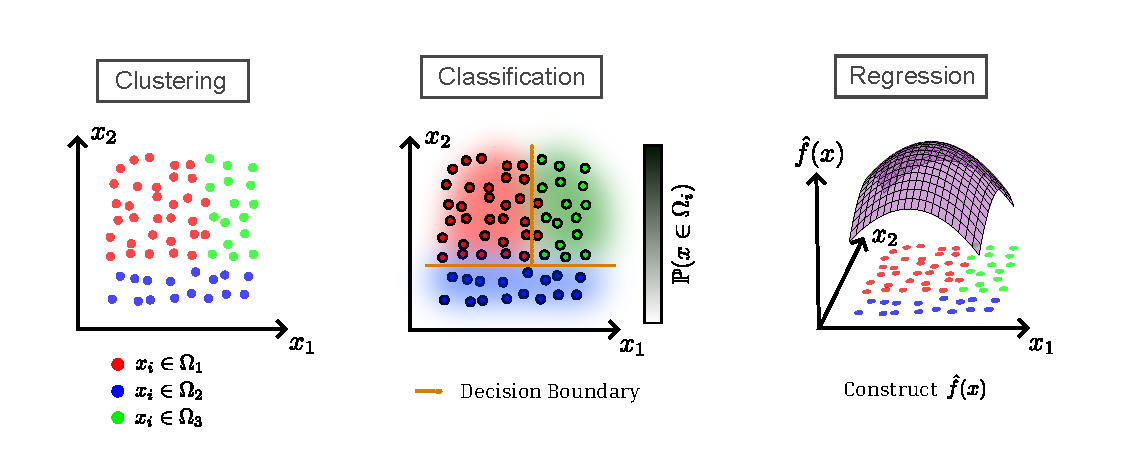
\includegraphics[width=\textwidth]{figures/sota_2/subtasks.pdf}
    \caption{Schematic representation of the three sub-tasks for building a piecewise surrogate model: (i) Clustering, (ii) Classification and (iii) Regression.}
    \label{fig:sota_2:clustering}
\end{figure}

Figure~\ref{fig:sota_2:clustering} provides a schematic representation of these three sub-tasks. \blue{As evident from the previous discussion, a good clustering of the training data $\data$ is crucial for the success of the piecewise surrogate model. Indeed, regression and classification are both common tasks in the field of machine learning, and their precision and accuracy can be easily tested by means of standard metrics, such as \gls{loo}-\gls{cv}. On the other hand, clustering is a more complex task, as it is an unsupervised learning problem.}

\smallskip
\blue{A key aspect that we want to stress is that we can't define how \textit{good} a clustering solution is without considering the regression task. Consider, for example, two cases, one in which we are using degree-1 polynomials and one in which we are using \glspl{gp} with \gls{rbf} covariances as local surrogate models. In the first case, a good clustering solution is one that identifies clusters in which the function $f$ is approximately linear, while in the second case, a good clustering solution is one that identifies regions in which the function $f$ is smooth. In other words, the quality of a clustering solution is not an intrinsic property of the clustering itself, but it depends on the regression task that we want to perform. This is a crucial point that is often overlooked in the literature, and it highlights the importance of jointly solving the clustering and regression problems when building a piecewise surrogate model.}

\smallskip
\blue{In the next section, we will discuss some of the existing approaches for building a piecewise surrogate model, focusing on how they combine clustering, classification and regression to identify the partition $\mathcal{P}$ of the input space $\Omega$ and to train the local surrogate models $\tilde{f}(\cdot; \boldsymbol{\beta}_l)$ for each cluster $l$.}

\subsection{Existing Approaches for Piecewise Surrogate Modeling}

A popular clustering technique is K-means~\cite{lloyd1982least}. Suppose we want to cluster the training data $\data$ into $K$ clusters. K-means starts by randomly initializing $K$ cluster centroids $\{\mathbf{c}_k \in \data\}_{k=1}^K$, and then iteratively assigns each training point $\mathbf{d}_i$ to the nearest centroid, and updates the centroids based on the mean of the assigned points.

\begin{algorithm}[htbp]
\caption{K-means clustering}
\label{alg:kmean}
\begin{algorithmic}[1]
\State \textbf{Input:} Data points $\data = \{\mathbf{d}_i\}_{i=1}^{\nobs}$, number of clusters $K$
\State Initialize $K$ centroids $\{\mathbf{c}_k\}_{k=1}^K$ (e.g., randomly select $K$ data points)
\Repeat
    \State Assign each point $\mathbf{d}_i$ to the nearest centroid:
    \begin{equation*}
        z_i \gets \arg\min_{k} \|\mathbf{d}_i - \mathbf{c}_k\|^2
    \end{equation*}
    \State Update each centroid $\mathbf{c}_k$ as the mean of assigned points:
    \begin{equation*}
        \mathbf{c}_k \gets \frac{1}{N_k} \sum_{i: z_i = k} \mathbf{d}_i
    \end{equation*}
\Until{cluster assignments $\mathbf{z}$ do not change}
\State \textbf{Output:} Cluster labels $\mathbf{z}$ and centroids $\{\mathbf{c}_k\}$
\end{algorithmic}
\end{algorithm}

Alg.~\ref{alg:kmean} provides a pseudo-code for the K-means clustering algorithm. The question of how to choose the number of clusters $K$ is a well-known problem in the field of clustering. \blue{A common approach is to use the Elbow method, which consists in plotting the \gls{wcss} as a function of $K$ and looking for the point where the decrease in \gls{wcss} starts to level off, forming an \textit{elbow} in the plot. Another approach is to use the Silhouette score, which measures how similar a point is to its own cluster compared to other clusters. The optimal number of clusters is often chosen as the one that maximizes the average Silhouette score across all points~\cite{kmeans1, kmeans2}.}

\smallskip
The seminal work of~\cite{kim2005} proposes to use a Bayesian approach in which adding, removing or moving a centroid is accepted if it leads to an improvement in the marginal likelihood of the surrogate model. This approach solves the clustering problem jointly with the regression problem, as the clustering is informed by the surrogate model. In~\cite{Sudret2023, Sudret2019} clustering is done using a \gls{gmm}, which corresponds to a soft (probabilistic) version of K-means. The number of clusters is automatically selected using a \gls{dp} prior, \blue{which allows for the data to determine the optimal number. A \gls{svm} is then used to learn the classifier, which is trained using the cluster labels obtained from the \gls{gmm}}. Their approach was also adapted by~\cite{Palar2024}, who used it to build explainable surrogate models for the analysis of stochastic re-entry trajectories using \glspl{pce}. 

\smallskip
If clustering is done using a K-means algorithm, then a natural choice for the classifier is a Voronoi tessellation of the input space $\Omega$, where each subdomain $\Omega_l$ is defined as the set of points that are closer to the centroid $\mathbf{c}_l$ than to any other centroid. This is the approach used by~\cite{kim2005}, although they treat it in a Bayesian way by averaging over many different tessellations.

\smallskip
The work of~\cite{Gramacy2008} introduced the idea of using tree-based methods to partition the input space $\Omega$ into subdomains for \gls{gp} regression. Tree based methods start by recursively splitting the input space $\Omega$ along a certain dimension, based on a certain criterion. For example, in~\cite{Bilionis2012} the authors propose to split a node into two child nodes whenever its contribution to the total predictive uncertainty is above a certain threshold.


\begin{algorithm}[htbp]
\caption{\blue{Pseudo Code for a Recursive Tree Partitioning}}
\label{alg:tree_compact}
\begin{algorithmic}[1]
\State \textbf{Input:} Domain $\Omega$, Data $\mathcal{D}$, Error function $\mathcal{E}(\cdot)$
\vspace{0.1cm}
\Function{Partition}{$\Omega, \mathcal{D}$}
    \If{stopping criteria met (e.g., $\mathcal{E}(\mathcal{D}) \le \epsilon$)} 
        \State \Return $\{\Omega\}$
    \EndIf
    
    \State Find optimal feature $j^*$ and split point $s^*$ that maximize error reduction:
    \State \quad $(j^*, s^*) \gets \arg\max_{j, s} \left[ \mathcal{E}(\mathcal{D}) - \sum_{k \in \{L, R\}} \frac{|\mathcal{D}_k|}{|\mathcal{D}|} \mathcal{E}(\mathcal{D}_k) \right]$
    
    \State \Return \Call{Partition}{$\Omega_{L}, \mathcal{D}_{L}$} $\cup$ \Call{Partition}{$\Omega_{R}, \mathcal{D}_{R}$}
\EndFunction
\State \textbf{Output:} $\mathcal{P} \gets$ \Call{Partition}{$\Omega, \mathcal{D}$}
\end{algorithmic}
\end{algorithm}

\blue{Algorithm~\ref{alg:tree_compact} outlines the general recursive procedure for tree-based space partitioning. Given an initial input domain $\Omega$ and an associated training dataset $\mathcal{D}$, the algorithm iteratively splits the space by identifying an optimal splitting dimension $j^* \in \{1, \ldots, d_x\}$ and a corresponding threshold $s^*$. This optimal split axis is determined by maximizing the reduction in an error metric $\mathcal{E}(\cdot)$ across the resulting left and right partitions. The error metric could be the \gls{mse} or some function of the predictive variance. The recursive splitting continues until a predefined stopping criterion is satisfied. The result is a partition $\mathcal{P}$ of the input space $\Omega$ into subdomains, which can then be used to train local surrogate models and automatically make predictions.}

\smallskip
\red{The use of tree-based methods is also popular in the context of \gls{pce}~\cite{megpc}. In particular, practitioners use~\gls{megpc} in which an algorithm like Algorithm~\ref{alg:tree_compact} is used to build a partition of the random input space. In this approach, the domain is recursively decomposed whenever the local error contribution, typically measured by the decay rate of the relative error weighted by the element's size, exceeds a predefined threshold. By dynamically identifying and bisecting the most sensitive random dimension, the algorithm builds an adaptive, tree-like mesh of subdomains. Within each newly generated child element, a localized polynomial chaos expansion is applied, effectively scaling down the local degree of random perturbation.}


\smallskip
\blue{The main disadvantage of tree-based methods is that the shape of the partition $\mathcal{P}$ is constrained by the axis-aligned splits, which may not be sufficient to capture complex, non-linear decision boundaries. This can lead to suboptimal partitions and therefore suboptimal surrogate models. A possible solution to this problem is found by forest approaches~\cite{das2018fast}, in which multiple trees are trained on different subsets of the data and the final prediction is obtained by averaging the predictions of the individual trees. This allows for more flexible partitions, as the combination of multiple trees can capture more complex decision boundaries. However, this comes at the cost of increased computational complexity and reduced interpretability of the surrogate model.}

\smallskip
\red{An alternative approach to overcoming the limitations of rigid, axis-aligned partitions is to explicitly detect and isolate the discontinuity using a flexible, unstructured boundary. Rather than relying on recursive bounding boxes or ensemble averaging, the work of~\cite{archibald2006polynomial} demonstrated that the exact coordinates of a jump or edge can be mathematically pinpointed using polynomial annihilation, a technique that exploits the local oscillatory behavior of polynomials (the Gibbs phenomenon) near sharp transitions. Building upon this localized detection, the work of~\cite{gorodetsky2014efficient} proposed an efficient framework that feeds these identified edge points into a \gls{svm} classifier. The \gls{svm} constructs a smooth, non-linear decision boundary that cleanly slices the domain into piecewise smooth regions. By replacing the structured grid of a standard tree with a custom machine-learning boundary, this method effectively isolates complex discontinuities and restores the spectral convergence of the polynomial approximation with significantly fewer computational resources.}

\smallskip
\blue{Another interesting approach, popular in the context of \gls{gpr}, is to use a \gls{moe} model~\cite{GPmixture}, in which the classifier is trained jointly with the local surrogate model. In a standard \gls{moe} framework, the global predictive distribution $\mathrm{p}(y \mid \mathbf{x})$ is defined as a mixture of $K$ local expert models, weighted by a classifier (called the gating network) that assigns probabilities to each expert based on the input $\mathbf{x}$. Formally, the predictive distribution can be expressed as:}

\begin{equation}
    \mathrm{p}(y \mid \mathbf{x}) = \sum_{k=1}^K \mathbb{P}_{\mathrm{CLS}}(z=k \mid \mathbf{x}; \boldsymbol{\gamma}) \, \mathrm{p}(y \mid \mathbf{x}, \boldsymbol{\beta}_k)
    \label{eq:sota_2:mixture_reconstruction}
\end{equation}

\blue{where $\mathbb{P}_{\mathrm{CLS}}(z=k \mid \mathbf{x}; \boldsymbol{\gamma})$ is the probability assigned by the gating network to expert $k$ for input $\mathbf{x}$, parameterized by $\boldsymbol{\gamma}$, and $\mathrm{p}(y \mid \mathbf{x}, \boldsymbol{\beta}_k)$ is the predictive distribution of the local surrogate model (expert) $k$, parameterized by $\boldsymbol{\beta}_k$. The gating network is typically implemented as a density estimator, which allows it to capture complex, non-linear decision boundaries in the input space.}

\smallskip
\blue{The main advantage of the \gls{moe} approach is that it allows for a joint optimization of the clustering, classification and regression tasks, as the gating network and the local surrogate models are trained together using an \gls{em} algorithm. This is a complex and multidimensional sampling problem, as the \gls{em} needs to sample the space of all possible $\mathbf{z}, \boldsymbol{\gamma}, \boldsymbol{\beta}$, but it has the potential to yield a more accurate and robust piecewise surrogate model.}


\subsection{Reconstruction of the Piecewise Surrogate Model}

\blue{Before discussing the limitations of the state of the art, we want to briefly address three recombination techniques that are commonly used in the literature to reconstruct the piecewise surrogate model from the local surrogate models and the classifier. These techniques are: (i) Piecewise Reconstruction, (ii) Soft Reconstruction and (iii) Mixture Reconstruction. The Soft and Mixture reconstructions are schematically represented in Fig.~\ref{fig:sota_2:reconstructions}.}

\begin{figure}[htbp]
    \centering
    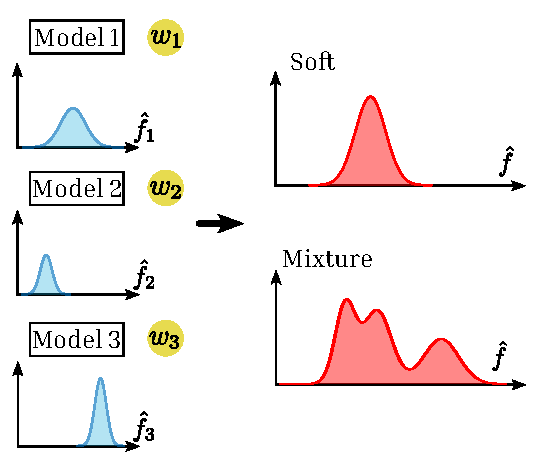
\includegraphics[width=0.6\textwidth]{figures/clustering/reconstruction.pdf}
    \caption{Schematic representation of the soft and mixture reconstructions of the surrogate model.}
    \label{fig:sota_2:reconstructions}
\end{figure}


\subsubsection{Piecewise Reconstruction}
\blue{As hinted before}, the piecewise reconstruction in Eq.~\eqref{eq:sota_2:f_piece_surr} can be readily obtained by using the classifier to define the partition $\mathcal{P}$ of the input space $\Omega$, i.e., by defining $\Omega_l = \{\bx \in \Omega : c(\bx; \boldsymbol{\gamma}) = l\}$. 

\smallskip
\blue{The main advantage of the piecewise reconstruction is that it allows for a very accurate representation of the function $f$, as it uses the local surrogate model $\tilde{f}_l$ that is specifically trained for the subdomain $\Omega_l$ to make predictions for any input $\bx \in \Omega_l$. The main disadvantage of the piecewise reconstruction is that it can lead to discontinuities in the predictions at the boundaries between subdomains, which can be problematic in some applications. Furthermore, if data is mis-clustered or if the classifier is uncertain about which model to choose, the piecewise reconstruction can lead to large errors in the predictions.}

\subsubsection{Soft Reconstruction}
To address these issues, one can use a \textit{soft reconstruction}~\cite{Sudret2023} of the surrogate model, in which the prediction for a new input $\bx$ is given by a weighted average of the predictions of the local surrogate models,

\begin{equation}
    \tilde{f}(\mathbf{x}; \boldsymbol{\beta}, \boldsymbol{\gamma}) = \sum_{l=1}^{L} w_l \ \tilde{f}_l(\bx; \boldsymbol{\beta}_l) \;,
    \label{eq:sota_2:soft_reconstruction}
\end{equation}

where $w_l : \sum_{l=1}^L w_l = 1$ are some weights. Notice that Eq.~\eqref{eq:sota_2:soft_reconstruction} is a generalization of the piecewise reconstruction, which can be recovered by setting $w_l = \mathbb{I}_{\Omega_l}(\bx)$. A common choice for the weights is to set them proportional to the classifier probability of belonging to each cluster, i.e., $w_l \propto \mathbb{P}_{\mathrm{CLS}}(\bx \in \Omega_l)$. 

\smallskip
\blue{A peculiarity of the soft reconstruction is that if the local surrogate models predictive distributions are Gaussian $\normalpdf(\mu_l, \sigma_l^2)$, then the soft reconstruction is also a Gaussian distribution $\normalpdf(\mu, \sigma^2)$, with mean $\mu = \sum_{l=1}^L w_l \mu_l$ and variance $\sigma^2 = \sum_{l=1}^L w_l^2 \sigma_l^2$. This means that the soft reconstruction can be seen as a Gaussian distribution that averages the predictions of the local surrogate models according to the weights $w_l$. This is illustrated in Fig.~\ref{fig:sota_2:reconstructions}, where the soft reconstruction is shown as a Gaussian distribution that averages the predictions of the local surrogate models.}

\smallskip
\blue{The biggest disadvantage of the soft reconstruction is that it does not yield an accurate representation of the uncertainty in the predictions. Indeed, if two local surrogate models $\tilde{f}_l$ and $\tilde{f}_{l'}$ are very certain on their prediction (small variance) but they predict very different values for the same input $\bx$, the soft reconstruction will give a narrow distribution around the average of the two predictions, which can be very far from the true value of $f(\bx)$. Furthermore, consider the case in which the classifier is uncertain about which model to choose and assigns equal weights to all local models (i.e., $w_l = 1/L$ for all $l$), assuming that the variance is the same for all local surrogate models (i.e., $\sigma_l^2 = \sigma^2$ for all $l$), the variance of the soft reconstruction will be $\sigma^2 / L$, which is smaller than the variance of each local surrogate model, thus leading to an underestimation of the uncertainty in the predictions.}


\subsubsection{Mixture Reconstruction}

\blue{The mixture reconstruction, popular in \gls{moe} models~\cite{GPmixture, park2025}, solves the issues of the soft reconstruction by building a mixture distribution from the predictive distributions of the local surrogate models, weighted by the classifier probabilities. The result is the same expression as the one in Eq.~\eqref{eq:sota_2:mixture_reconstruction}. This is illustrated in Fig.~\ref{fig:sota_2:reconstructions}, where the mixture reconstruction is shown as a mixture of Gaussian distributions that mixes the distributions of the local surrogate models according to the weights $w_l$.}

\smallskip
The advantage of the mixture reconstruction is that it yields a more accurate representation of the uncertainty in the predictions. \blue{Indeed, while the mean is simply the average of the local means (as in the Soft Reconstruction case), the variance is given by the mixture variance formula:}

\begin{equation}
    \mathbb{V}_{\tilde{f}}[\tilde{f}(\bx)] = \sum_{l=1}^L w_l \left( \mathbb{V}_{\tilde{f}_l}[\tilde{f}_l(\bx)] + (\mathbb{E}_{\tilde{f}_l}[\tilde{f}_l(\bx)] - \mathbb{E}_{\tilde{f}}[\tilde{f}(\bx)])^2 \right) \;.
    \label{eq:sota_2:mixture_var}
\end{equation}

\blue{Notice that Eq.~\eqref{eq:sota_2:mixture_var} contains two terms: the first term is the weighted average of the variances of the local surrogate models $\mathbb{V}_{\tilde{f}_l}[\tilde{f}_l]$, called \textit{intrinsic uncertainty}, and the second term is the weighted average of the squared differences between the means of the local surrogate models $\mathbb{E}_{\tilde{f}_l}[\tilde{f}_l]$ and the mean of the overall surrogate model $\mathbb{E}_{\tilde{f}}[\tilde{f}]$. This second term captures the uncertainty due to the classification task, and it is often referred to as the \textit{model uncertainty}. Notice that, contrary to the soft prediction, the intrinsic uncertainty does not suffer from the same underestimation issue, and assuming that the classifier is uncertain about which model to choose and assigns equal weights to all local models (i.e., $w_l = 1/L$ for all $l$), the intrinsic variance of the mixture will be $\sigma^2$, and not $\sigma^2 / L$ as in the soft reconstruction case.}


\subsection{Limitations of the State-of-the-Art Approaches}

\blue{Many techniques have been proposed in the literature to build piecewise surrogate models, and they have been shown to be effective in many cases. However, they all share some common limitations.}

\smallskip
\blue{First, techniques that rely on K-means or tree-based methods for clustering and classification are limited by the shape of the clusters they can capture. K-means can only capture convex clusters, while tree-based methods can only capture axis-aligned splits. This can be a significant limitation when dealing with complex, non-linear decision boundaries.}

\smallskip
\blue{The above limitation is addressed by using a model-based clustering approach, such as the \gls{moe} model~\cite{GPmixture}, in which the clustering, classification and regression tasks are solved jointly. However, training \gls{moe} models can be computationally expensive and may require careful tuning of the hyperparameters~\cite{Teemu2025}. We also note that \gls{moe} models require the development and implementation of specialized sampling techniques, and do not leverage existing and commonly used optimization or hyperparameter selection techniques.}

\smallskip
\blue{Finally, the approach of~\cite{Sudret2023, Palar2024} is very appealing, as it addresses the computational cost of \gls{moe} models by solving the clustering, classification and regression tasks independently. However, its strength is also its weakness, as the clustering and classification tasks are solved independently of the regression task, which can lead to suboptimal solutions. Indeed, the clustering obtained from their \gls{dp} prior is not informed by the performance of the surrogate model, and may lead to the presence of some mis-clustered points, as will be shown in our numerical experiments in Chapter~\ref{sec:clustering}.}

\smallskip
\blue{The goal of this work is to address the above limitations by proposing a model-based clustering approach that solves the clustering, classification and regression tasks jointly, while remaining agnostic to the choice of surrogate model and classifier. To do that, we will frame the problem as a joint optimization problem over the cluster labels $\mathbf{z}$, the classifier hyperparameters $\boldsymbol{\gamma}$ and the surrogate model hyperparameters $\boldsymbol{\beta}$, and we will solve this optimization problem using an alternating optimization approach. Such an approach allows us to leverage existing optimization techniques and software for hyperparameter ($\boldsymbol{\beta}$ and $\boldsymbol{\gamma}$) tuning, and to provide theoretical guarantees on the convergence of the algorithm to a local optimum.}
